\documentclass{article}

\usepackage[utf8]{inputenc}
\usepackage{graphicx}
\usepackage{booktabs}
\usepackage{subcaption}

\title{Project report DD2360}
\author{Jacob Wahlgren \texttt{<jacobwah@kth.se>} \\ Expected grade: A}

\begin{document}

\maketitle

\section{Introduction}
% Background on the problem
%
\section{Methodology}
% Explain implementation

\section{Experimental setup}
% Gpu platform, software and hardware, tools

\section{Results}
% Validation, performance

Visual inspection of the generated images using the \verb|display| command
validated the results. Example images are shown in figure \ref{fig:output}.

The performance comparison of the CPU and GPU versions showed that the GPU
vastly outperforms the CPU version on this task. The difference was more
noticeable at larger image dimensions. In fact, results were not obtained for
the CPU version above image dimension 1000 since it was too slow. The results
are presented in figure \ref{fig:cpu}, were the Quadra K240 fwrite 8x8
configuration is used to represent the GPU.

We evaluate the performance of different GPU configurations at image size
1000x1000 (normal) and 100000x100000 (huge).

\begin{figure}
    \begin{subfigure}{0.5\linewidth}
        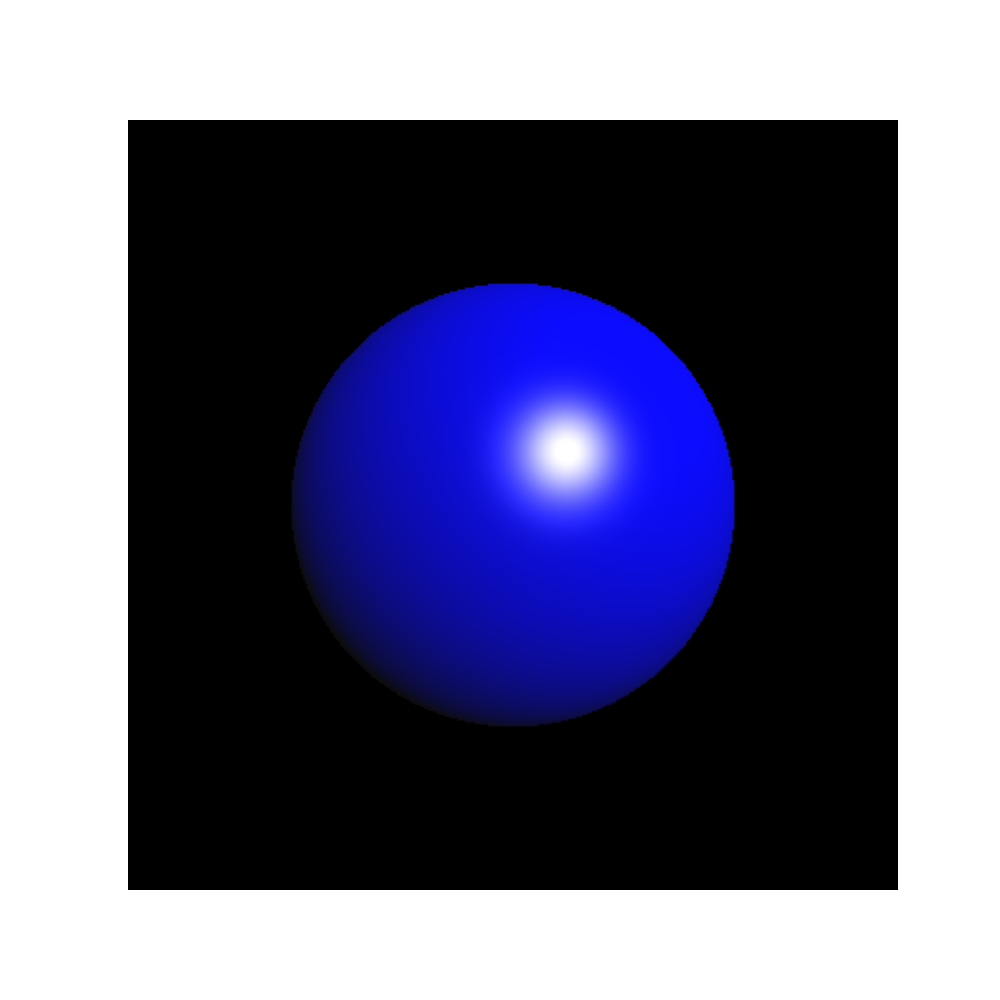
\includegraphics[width=\linewidth]{../raytracing_py.png}
        \caption{CPU image.}
    \end{subfigure}
    \begin{subfigure}{0.5\linewidth}
        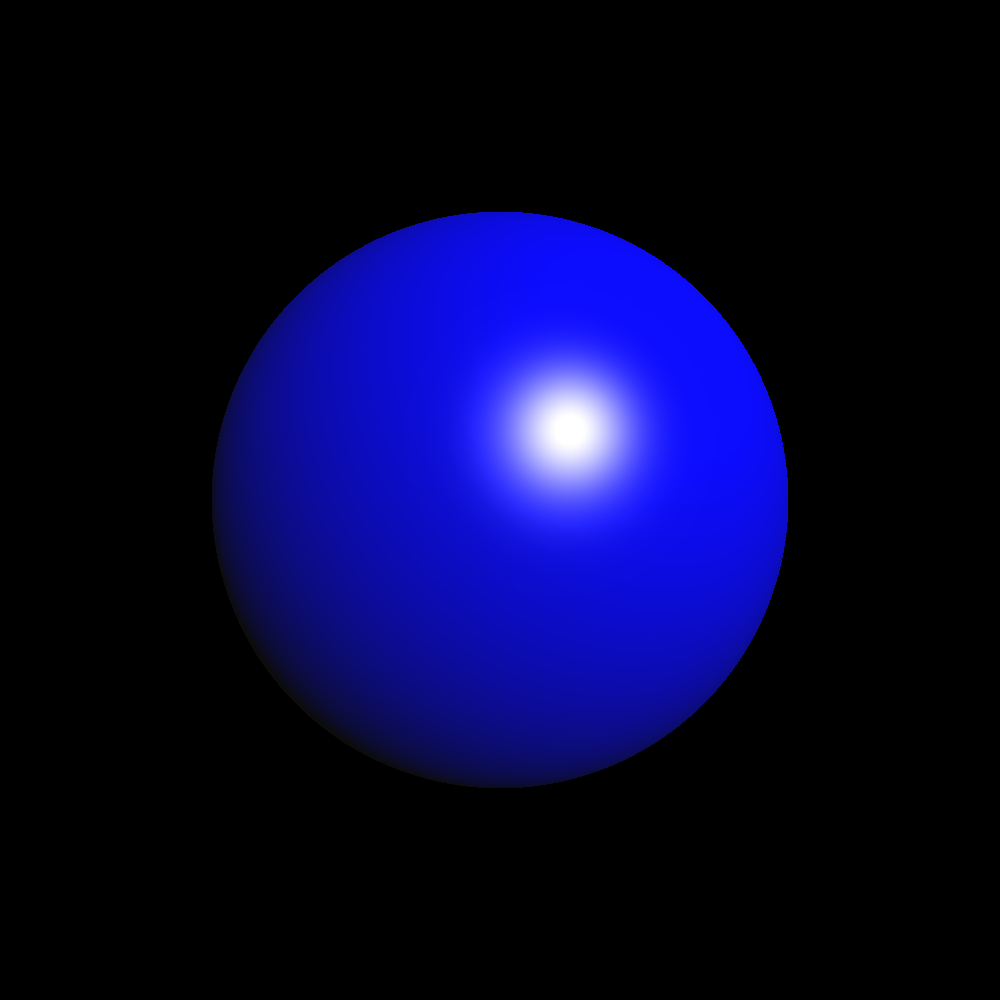
\includegraphics[width=\linewidth]{output.png}
        \caption{GPU image.}
    \end{subfigure}
    \caption{Sample output images. Note that the CPU version generates a white
    border around the image.}
    \label{fig:output}
\end{figure}

\begin{figure}
    \centering
    \includegraphics{../fig/cpu.pdf}
    \caption{Performance comparison between Python CPU version and fwrite 8x8
    GPU version, average of 10 runs. Both run on Tegner thin nodes.}
    \label{fig:cpu}
\end{figure}

\begin{figure}
    \begin{subfigure}{\linewidth}
        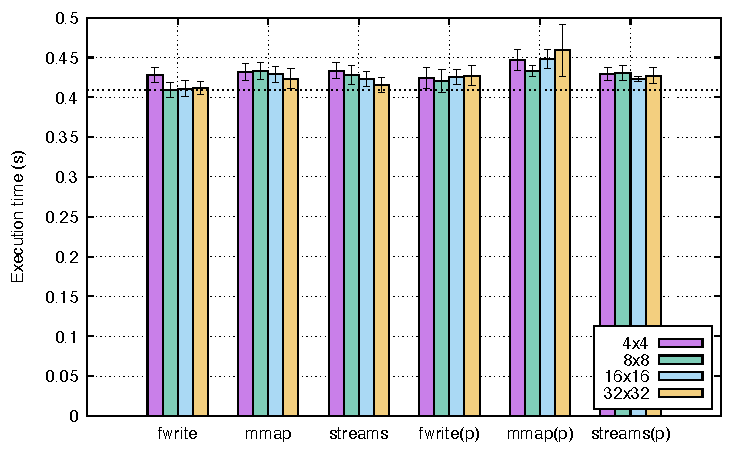
\includegraphics{../fig/sm30-1000.pdf}
        \caption{NVIDIA Quadro K240}
    \end{subfigure}
    \begin{subfigure}{\linewidth}
        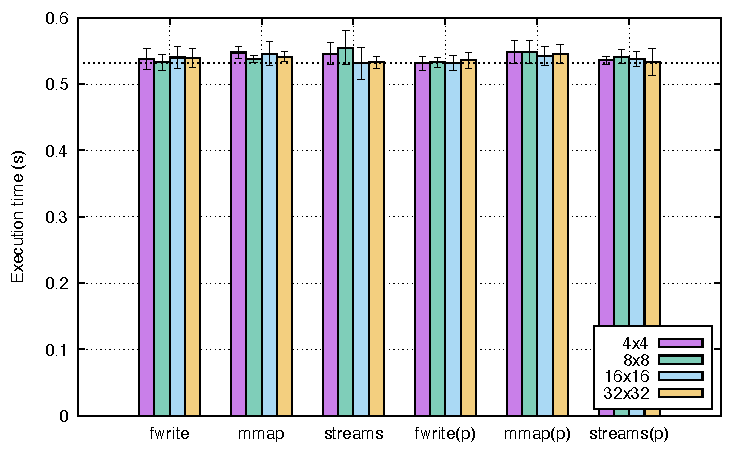
\includegraphics{../fig/sm37-1000.pdf}
        \caption{NVIDIA Tesla K80}
    \end{subfigure}
    \caption{Performance results for 1000x1000 image with various block sizes. Bars show average, whiskers show
    standard deviation.}
\end{figure}

\begin{figure}
    \begin{subfigure}{\linewidth}
        \includegraphics{../fig/sm30-100000.pdf}
        \caption{NVIDIA Quadro K240}
    \end{subfigure}
    \begin{subfigure}{\linewidth}
        %\includegraphics{../fig/sm37-100000.pdf}
        \caption{NVIDIA Tesla K80}
    \end{subfigure}
    \caption{Performance results for 100000x100000 image with various block
        sizes. Bars show average, whiskers show
    standard deviation.}
\end{figure}

\section{Discussion and conclusion}
% Discuss performance results
% Challenges and limitations
% Optimizations

The specular highlight in output images from the CPU and the GPU versions are
slightly different. This is likely caused by using different floating
point precision (double in Python, single in CUDA).

\end{document}
